\section{Appendix}

Appendices (optional) are placed at the end of the report. They contain information that is not essential to understanding the work. However, they are included to ensure a complete report. They could include a glossary, a list of acronyms, etc.~\cite{melot2008elements}.

\section{Writing Instructions}

Writing instructions for the state-of-the-art.

\begin{itemize}
    \item Although highly recommended, use of \LaTeX is not mandatory for the state-of-the-art.
    \item Writing in scientific English is recommended, but using scientific French is possible under the permission of your advisor. In this latter case, it is recommended to include a bilingual glossary, since the translation of scientific terms in French is often not standardized.  
    \item Spelling, syntax, punctuation are very important! 
    \begin{itemize}
        \item Minus 0.5 points for every 5 mistakes (including spelling, grammar, syntax and punctuation).
        \item Use and abuse automatic spellchecker, and have yourself proofread!
    \end{itemize}
\end{itemize}

\section{Latex Cheat Sheet}

This cheat sheet is an adaptation of the ACM Official Article Templates~\cite{acm2023templates}. You can also consult Vincent Englebert's guide~\cite{englebert2023latex} and Overleaf's tutorials~\cite{overleaf2023latex}.

\subsection{Introduction}

This section is a guide to the process of preparing your manuscript in \LaTeX. Besides the template itself, it contains instructions and examples relating to the use of the main \LaTeX\  functionalities required to produce your manuscript. It is mainly based on ACM proceedings templates\footnote{\url{https://www.acm.org/publications/proceedings-template}} and Overleaf tutorial \footnote{\url{https://www.overleaf.com/learn}}. Overleaf tutorial is also a great resource to help you to deepen into what is presented here.

\subsection{Sectioning Commands}

Your work should use standard \LaTeX\ sectioning commands: \verb|section|, \verb|subsection|, \verb|subsubsection|, and \verb|paragraph|. They should be numbered; do not remove the numbering from the commands.

Simulating a sectioning command by setting the first word or words of a paragraph in boldface or italicized text is not recommended.

\subsection{Tables}

The template includes the ``\verb|booktabs|'' package --- \url{https://ctan.org/pkg/booktabs} --- for preparing high-quality tables.

Table captions are placed {\itshape above} the table.

Because tables cannot be split across pages, the best placement for them is typically the top of the page nearest their initial cite.  To ensure this proper ``floating'' placement of tables, use the environment \textbf{table} to enclose the table's contents and the table caption.  The contents of the table itself must go in the \textbf{tabular} environment, to be aligned properly in rows and columns, with the desired horizontal and vertical rules..

Immediately following this sentence is the point at which Table~\ref{tab:freq} is included in the input file; compare the placement of the table here with the table in the printed output of this document.

\begin{table}[ht]
	\centering
	\caption{Frequency of Special Characters}
	\label{tab:freq}
	\begin{tabular}{ccl}
		\toprule
		Non-English or Math&Frequency&Comments\\
		\midrule
		\O & 1 in 1,000& For Swedish names\\
		$\pi$ & 1 in 5& Common in math\\
		\$ & 4 in 5 & Used in business\\
		$\Psi^2_1$ & 1 in 40,000& Unexplained usage\\
		\bottomrule
	\end{tabular}
\end{table}

Always use midrule to separate table header rows from data rows, and use it only for this purpose. This enables assistive technologies to recognise table headers and support their users in navigating tables more easily.

\subsection{Math Equations}

You may want to display math equations in three distinct styles: inline, numbered or non-numbered display.  Each of the three are discussed in the next sections.

\subsubsection{Inline (In-text) Equations}

A formula that appears in the running text is called an inline or in-text formula.  It is produced by the \textbf{math} environment, which can be invoked with the usual \texttt{{\char'134}begin\,\ldots{\char'134}end} construction or with the short form \texttt{\$\,\ldots\$}. You can use any of the symbols and structures, from $\alpha$ to $\omega$, available in \LaTeX~\cite{Lamport:LaTeX}; this section will simply show a few examples of in-text equations in context. Notice how this equation:
\begin{math}
	\lim_{n\rightarrow \infty}x=0
\end{math},
set here in in-line math style, looks slightly different when set in display style.  (See next section).

\subsubsection{Display Equations}

A numbered display equation---one set off by vertical space from the text and centered horizontally---is produced by the \textbf{equation} environment. An unnumbered display equation is produced by the \textbf{displaymath} environment.

Again, in either environment, you can use any of the symbols and structures available in \LaTeX\@; this section will just give a couple of examples of display equations in context.  First, consider the
equation, shown as an inline equation above:
\begin{equation}
	\lim_{n\rightarrow \infty}x=0
\end{equation}
Notice how it is formatted somewhat differently in the \textbf{displaymath} environment.  Now, we'll enter an unnumbered equation:
\begin{displaymath}
	\sum_{i=0}^{\infty} x + 1
\end{displaymath}
and follow it with another numbered equation:
\begin{equation}
	\sum_{i=0}^{\infty}x_i=\int_{0}^{\pi+2} f
\end{equation}
just to demonstrate \LaTeX's able handling of numbering.

\subsection{Figures}

The ``\verb|figure|'' environment should be used for figures. One or more images can be placed within a figure. If your figure contains third-party material, you must clearly identify it as such, as shown in the example below.
\begin{figure}[ht]
	\centering
	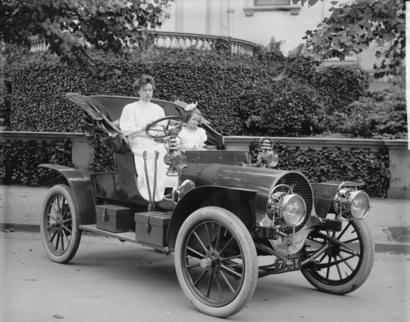
\includegraphics[width=\linewidth]{figures/sample-franklin}
	\caption{1907 Franklin Model D roadster. Photograph by Harris \&
		Ewing, Inc. [Public domain], via Wikimedia
		Commons.}
\end{figure}

Your figures should contain a caption which describes the figure to the reader.

Figure captions are placed {\itshape below} the figure.

Every figure should also have a figure description unless it is purely decorative. These descriptions convey what’s in the image to someone who cannot see it. They are also used by search engine crawlers for indexing images, and when images cannot be loaded.

\subsection{Citations and Bibliographies}

The use of BibTeX for the preparation and formatting of one's references is strongly recommended. Authors' names should be complete --- use full first names (``Donald E. Knuth'') not initials (``D. E. Knuth'') --- and the salient identifying features of a reference should be included: title, year, volume, number, pages, article DOI, etc.

The bibliography is included in your source document with these two commands, placed just before the \verb|\end{document}| command:
\begin{verbatim}
\bibliographystyle{unsrtnat}
\bibliography{bibfile}
\end{verbatim}
where ``\verb|bibfile|'' is the name, without the ``\verb|.bib|'' suffix, of the BibTeX file.

Some examples.  A paginated journal article \cite{Abril07}, an enumerated journal article \cite{Cohen07}, a reference to an entire issue \cite{JCohen96}, a monograph (whole book) \cite{Kosiur01}, a monograph/whole book in a series (see 2a in spec. document) \cite{Harel79}, a divisible-book such as an anthology or compilation \cite{Editor00} followed by the same example, however we only output the series if the volume number is given \cite{Editor00a} (so Editor00a's series should NOT be present since it has no vol. no.), a chapter in a divisible book \cite{Spector90}, a chapter in a divisible book in a series \cite{Douglass98}, a multi-volume work as book \cite{Knuth97}, a couple of articles in a proceedings (of a conference, symposium, workshop for example) (paginated proceedings article) \cite{Andler79, Hagerup1993}, a proceedings article with all possible elements \cite{Smith10}, an example of an enumerated proceedings article \cite{VanGundy07}, an informally published work \cite{Harel78}, a couple of preprints \cite{Bornmann2019, AnzarootPBM14}, a doctoral dissertation \cite{Clarkson85}, a master's thesis: \cite{anisi03}, an online document / world wide web resource \cite{Thornburg01, Ablamowicz07, Poker06}, a video game (Case 1) \cite{Obama08} and (Case 2) \cite{Novak03} and \cite{Lee05} and (Case 3) a patent \cite{JoeScientist001}, work accepted for publication \cite{rous08}, 'YYYYb'-test for prolific author \cite{SaeediMEJ10} and \cite{SaeediJETC10}. Other cites might contain 'duplicate' DOI and URLs (some SIAM articles) \cite{Kirschmer:2010:AEI:1958016.1958018}. Boris / Barbara Beeton: multi-volume works as books \cite{MR781536} and \cite{MR781537}. A couple of citations with DOIs: \cite{2004:ITE:1009386.1010128,Kirschmer:2010:AEI:1958016.1958018}. Online citations: \cite{TUGInstmem, Thornburg01, CTANacmart}. Artifacts: \cite{R} and \cite{UMassCitations}.

The bibliography is managed by the package \textbf{natbib}\footnote{\url{https://www.overleaf.com/learn/latex/Bibliography_management_with_natbib}}.
